%!TeX spellcheck = en-UK

\documentclass{tufte-handout}

\title{Pre-Proposal for a Capstone Project Intended to Satisfy the Requirements for an ALM in Digital Media Design at Harvard Extension School}

\author[Dave Morgan]{Dave Morgan}

%\date{28 March 2010} % without \date command, current date is supplied

%\usepackage{geometry}
% \geometry{showframe} % display margins for debugging page layout

\usepackage{graphicx} % allow embedded images
\setkeys{Gin}{width=\linewidth,totalheight=\textheight,keepaspectratio}
\graphicspath{{graphics/}} % set of paths to search for images
\usepackage{amsmath}  % extended mathematics
\usepackage{booktabs} % book-quality tables
\usepackage{units}    % non-stacked fractions and better unit spacing
\usepackage{multicol} % multiple column layout facilities
\usepackage{lipsum}   % filler text
\usepackage{fancyvrb} % extended verbatim environments
\fvset{fontsize=\normalsize}% default font size for fancy-verbatim environments




% Standardize command font styles and environments
\newcommand{\doccmd}[1]{\texttt{\textbackslash#1}}% command name -- adds backslash automatically
\newcommand{\docopt}[1]{\ensuremath{\langle}\textrm{\textit{#1}}\ensuremath{\rangle}}% optional command argument
\newcommand{\docarg}[1]{\textrm{\textit{#1}}}% (required) command argument
\newcommand{\docenv}[1]{\textsf{#1}}% environment name
\newcommand{\docpkg}[1]{\texttt{#1}}% package name
\newcommand{\doccls}[1]{\texttt{#1}}% document class name
\newcommand{\docclsopt}[1]{\texttt{#1}}% document class option name
\newenvironment{docspec}{\begin{quote}\noindent}{\end{quote}}% command specification environment

% my packages
\usepackage{ amssymb } % for \checkmark
% counter for resuming enumerated list numbers
\newcounter{resumeenumi}
\newcommand{\suspend}{\setcounter{resumeenumi}{\theenumi}}
\newcommand{\resume}{\setcounter{enumi}{\theresumeenumi}}

\newcommand\lb{\linebreak}
\newcommand\pars{\par\smallskip}
\newcommand\parm{\par\medskip}
\newcommand\parb{\par\bigskip}

%left flushed minipage
\newcommand{\minit}[2][0.8]{
	\begin{minipage}[t]{#1\columnwidth}
		\raggedright
		#2
	\end{minipage}
}

%left flushed minipage
\newcommand{\mini}[2][0.8]{
	\begin{minipage}[c]{#1\columnwidth}
		\raggedright
		#2
	\end{minipage}
}



% centered minipage with text \raggedright
%\cmini[width]{content}
\newcommand{\cmini}[2][0.8]{
	\begin{center}
		\begin{minipage}{#1\columnwidth}
			\raggedright
			#2
		\end{minipage}
	\end{center}
}

% get x and y coordinates from a tikz coordinate
%\gettikzxy{A}{\ax}{\ay}
\makeatletter
\providecommand{\gettikzxy}[3]{%
	\tikz@scan@one@point\pgfutil@firstofone#1\relax
	\edef#2{\the\pgf@x}%
	\edef#3{\the\pgf@y}%
}
\makeatother




\begin{document}
\raggedright
\maketitle% this prints the handout title, author, and date

\begin{abstract}
	% \noindent
	This document is a pre-proposal for Dave Morgan's capstone project, intended to satisfy requirements for an ALM in Digital Media Design at Harvard Extension School. The proposed project will involve the refactoring of a website authored a decade or so ago, and visible at \url{http://qwizm.org}.
	\parm\noindent
	Qwizm contains a number of quizzes or assignments, each comprised of questions having multiple parts. Input values to these questions are pseudo-randomized, and derived from a student ID number so that each student receives 'unique' question inputs. Answers are numerical.  To date, these questions have focused on problems in introductory engineering courses.
	\parm\noindent
	The aim of this refactoring is to make the site more accessible and user-friendly, and to take advantage of recent advances in technology allowed by HTML$5$, CSS$3$ and ES$6$. The proposed site will make it more convenient for instructors to create new questions and quizzes of their own and more convenient for students to use.

\end{abstract}


\section{Candidate Information}\label{sec:candidate}
\emph{First Name}: Dave \parm
\emph{Last Name}: Morgan \parm
\emph{ID}: 10823943 \parm
\emph{Education}: \\
\hspace{0.5cm}BSc. Applied Mathematics (2003), \\
\hspace{0.5cm}University of Calgary, Calgary, Alberta, Canada \parm
\hspace{0.5cm}BSc. Computer Science (2003), \\
\hspace{0.5cm}University of Calgary, Calgary, Alberta, Canada \parm
\emph{Current Employment}: Retired \parm
\emph{5-Year Deadline}: May, 2020 \parb

\section{Capstone Track}
	ALM in Digital Media Design

\section{\LARGE The Project}\label{sec:project}

\section{Background}\label{sec:background}
In 2005, I began teaching introductory engineering courses at a polytechnic offering two-year diploma programs for prospective engineering technologists. The courses I taught were problem-based and examples, exercises and assignments typically required multiple-step mathematical solutions. The mathematics is not advanced, usually little more than high-school algebra and trigonometry, but many students find it challenging.
\parm
Attempts to ensure independent student work on assigned 'homework' are an ongoing battle. Students are able to find solution manuals online for most textbooks, or may subscribe to services that supply solutions. Instructor-created problem-sets tend to encourage group work, with the strongest member of the group providing direction to those less able --- who may understand the process when it is presented to them but don't benefit from the exercise of thinking out a solution that builds from the same concepts yet is, perhaps only subtly, different from examples presented in class.
\parm
Many learning management systems (LMSes) offer question-types named 'arithmetical,' 'calculated' or equivalent, that provide pseudo-randomized question input values and marks the student submission based on that student's input values. For example, a simple question requiring the calculation of the area $A$ of a rectangle with length $L$ and height $H$ might have inputs (and corresponding calculated answer) for each student, as shown below:

% \begin{minipage}{\textwidth}
	\begin{table}[ht]
		\centering
		\fontfamily{ppl}\selectfont
		\small%
		\begin{tabular}{cr@{}lr@{}lr@{}lcr@{}l}
			\toprule
			Student & \multicolumn{2}{c}{$L\;\mathsf{(m)}$} & \multicolumn{2}{c}{$H\;\mathsf{(m)}$} & \multicolumn{2}{c}{$A\;\mathsf{(m^2)}$}                                                          \\
			\midrule
			Adams   & 2                       & .55                     & 1                       & .950 & 4 & .97  \textcolor{Green4}{\Large\checkmark}  \\
			Brown   & 1                       & .250                    & 0                       & .875 & 1 & .094  \textcolor{Green4}{\Large\checkmark} \\
			Clarke  & 4                       & .20                     & 1                       & .600 & 6 & .72  \textcolor{Green4}{\Large\checkmark}  \\
			\bottomrule
		\end{tabular}
		\caption{Possible sample inputs for length $L$ and height $H$, provided by an LMS for three different students, to find the area $A$ of a rectangle, along with solutions that would be marked correct by the LMS. }
	  % \label{tab:heading-styles}
	\end{table}
% \end{minipage}

\parm
Generally, questions in engineering courses are more complex and require several steps to reach the solution. In these cases, it is not often realistic to expect a student to arrive at a numerically accurate final answer without some feedback along the way. And, frequently, questions do not require a single final answer but several answers: such as calculating the tensile forces in bolts at the top and the bottom of an access hatch attached to a storage tank; or the determining of the reaction force in each of a number of connections in a rigid-member frame.\sidenote[][-3.8cm]{
	\raggedright
	A typcial engineering statics question requiring multiple numerical answers: \parm There is a frictionless roller at $E$ and pinned connections at $A$, $B$, $C$ and $F$. \\
	\hspace{-0.65cm}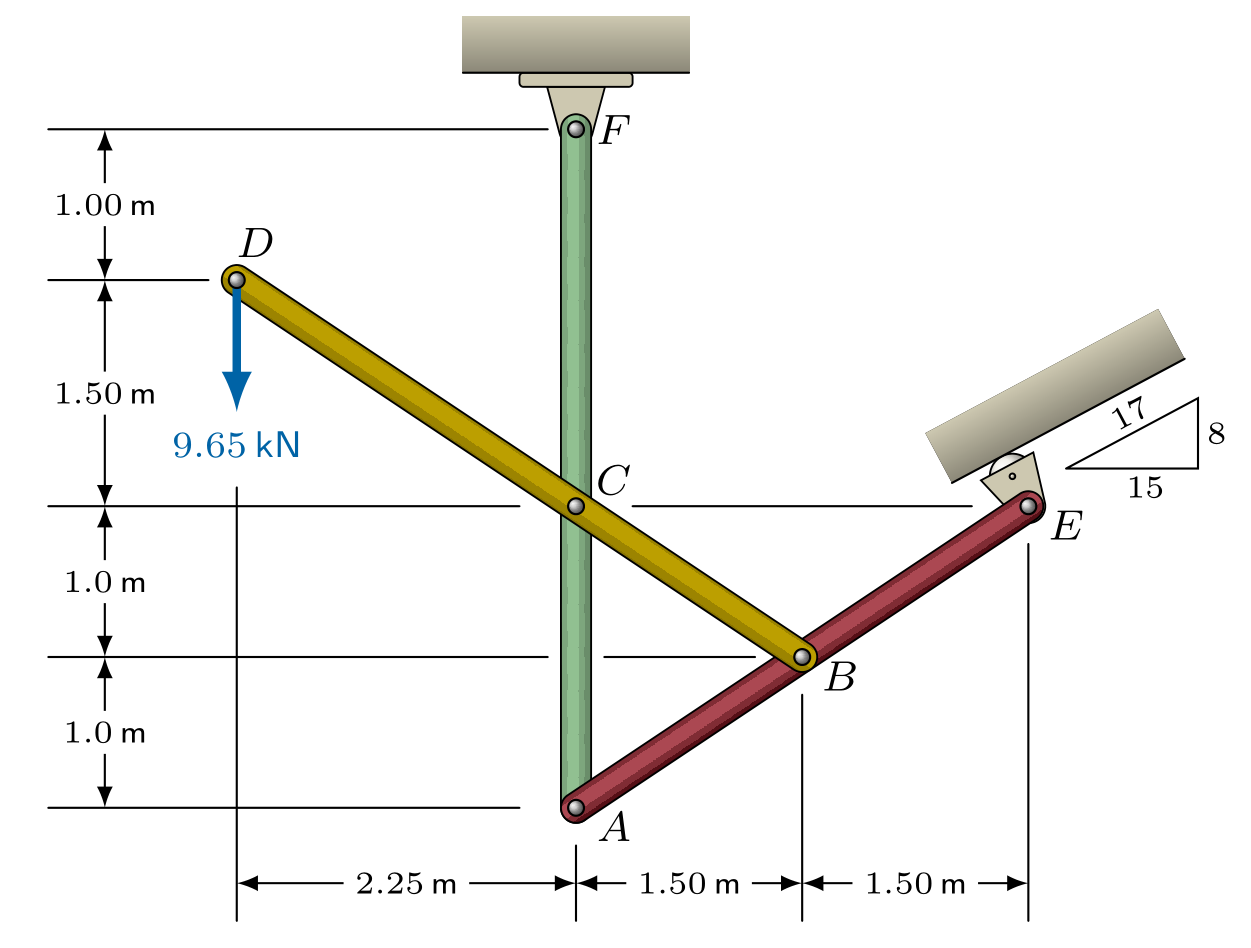
\includegraphics[width=1.25\linewidth]{includes/cf.png}\par\noindent
	Determine the magnitude of the reactions at all connections and the roller when a 9.65 kN force is applied vertically downwards at $D$.\vspace{0.5cm}
}
\newpage
LMSes don't generally offer question types that mark multiple answers although it does seem to be a much requested functionality (particularly on Canvas).\sidenote{https://community.canvaslms.com/thread/5891}\sidenote{https://app-community.canvaslms.com/ideas/8172-multiple-numerical-blanks}\sidenote{https://community.canvaslms.com/thread/30523-multiple-part-formula-question} Several years ago, the institution at which I worked was looking to switch to a new LMS; this multiple-answer functionality was strongly requested in the new LMS, not only by the engineering, and other, technology programs but also by several trade apprenticeship programs --- but this functionality was not available in the LMS eventually chosen. And the chosen LMS stripped any user-generated JavaScript from files so there was no way for users to implement a hack as had been managed in our previous LMS.
\parm
Moodle\sidenote{https://moodle.org} is a popular open-source LMS that offers an impressive list of question-types\sidenote{https://docs.moodle.org/37/en/Question\_types} but no mention of a random-input multiple-answer question-type. However, there is a Moodle plug-in (initiated in 2010 by Hon Wai Lau\sidenote{https://www.linkedin.com/in/hon-wai-lau-97508182}) that provides the required functionality.\sidenote{https://github.com/jmvedrine/moodle-qtype\_formulas} I have built a handful of sample questions\sidenote{{\scriptsize http://eduk8r.org/moodle/mod/quiz/view.php?id=24} \\User: learner, Password: Le@rner1} using this plug-in and consider it to be a realistic solution for those institutions that adopt Moodle as their LMS.
\parb
In 2008, I wrote a simple testing system,\sidenote{http://qwizm.org} partially as an exercise for learning JavaScript. I had a specific set of requirements:
\begin{enumerate}
	\setlength\itemsep{0.125em}
	\item Users have access to a modern browser.
	\item Questions are capable of 'marking' multiple parts (simply \textcolor{Green4}{\Large\checkmark}or \textcolor{Red2}{\textsf{X}}) to facilitate direction and progress through lengthy problem solutions.
	\item Individual parts can be assigned an arbitrary number of marks, each part contributing to the question total.
	\item Each question has randomized inputs, derived from the student's ID number. Logging in with the same ID number produces the same inputs.
	\item Randomized inputs are critical to these questions but sometimes we need more than a random value, e.g., we may need to pick a pipe randomly from a set of commercially available pipe sizes. Qwizm can accommodate this requirement (by picking an index randomly from an array of pipe sizes).
	\item All calculations are performed on the client side, in the browser. Nothing is stored between browser sessions. (Local storage in the browser was not then available.)
	\suspend
\end{enumerate}
\newpage
\begin{enumerate}
	\resume
	\item Input values are super-imposed on the diagram. For example, a length would be marked $3.25\,\textsf{m}$ on the diagram, rather than $x_1\,\textsf{m}$ marked on the diagram and $x_1=3.25\,\textsf{m}$ defined in the question statement. This functionality is not available in any LMS (to my knowledge) and is intended to remove one level of abstraction that can confuse the student.
	\item Student answers must be correct to three significant digits although 5 or more should be carried for intermediate calculations. (In 2010, I updated the marking function to check for four significant figures in answers where the first non-zero digit is a 1, to match the practice in our course textbooks.)
	\item There is a summary page, detailing all user entries, whether the entry is correct or not, and the marks earned for each part. Also, a total is calculated for the complete assignment.

\end{enumerate}

Initial student response to these Qwizm assignments was mixed. Some embraced it immediately, viewing it as 'guided-learning' and enjoying the instant feedback. Others struggled with the intentionally demanding accuracy (three, or four, significant digits, with no tolerance) required for a correct answer --- this followed the consistent pattern used in in-class examples. Initially, I had complaints of program 'bugs', i.e., Qwizm marking an answer wrong when the student was 'absolutely certain' that their answer was correct. For each class, I'd pick a particularly troublesome question and work through it on the board, demonstrating that it was indeed possible to get consistent \textcolor{Green4}{\Large\checkmark} marks the first time when sufficient attention was paid to significant figures.\sidenote{One topic, Forces Due to Static Fluids in an introductory course in Fluid Mechanics, can cause numerical problems The formula
\[ L_P-L_C = \frac{I_x}{L_C\cdot A} \]
is used to determine the very short distance, $L_P\!-\!L_C$. If the student uses $\frac{I_x}{L_C\cdot A}$ to calculate the value, the answer is given to the 5 or more required significant digits required for interim calculations. But, if the student calculates $L_P$ and $L_C$ first, to 5 significant digits, calculating $L_P\!-\!L_C$ may only have 2 or 3 significant digits.
\parm\noindent
For example, if $L_C\!=\!1.2345\,\textsf{m}$ and $L_P\!=\!1.2356\,\textsf{m}$, then \lb $L_P\!-\!L_C=0.0011\,\textsf{m}$ which has only two significant digits.
\parm\noindent
This can cause problems in achieving the 'correct' result later. The question creator should be aware of these numerical issues which are not directly related to Qwizm.}
\parm
Complaints diminished in number after these demonstrations, but students who aren't sufficiently accurate with their math often adopt a policy of trying adjacent final digits until they receive their own 'correct' checkmark.
\parm
(I have no remedy for this, due to other requirements I have chosen: to keep everything on the client side; and to allow students to reset the assignment --- a button that will simply clear local storage --- to start over, with a different ID number if desired.)

\section{Motivation}\label{sec:motivation}

Despite limitations, Qwizm has proved to be effective both as an assessment tool and as a learning tool. It continues to be used by the instructor who has taken over teaching my courses following my retirement from teaching. The refactoring proposed here is the first part of a larger project (beyond the scope of this capstone) to build a desktop application that will enable instructors with no programming knowledge to develop their own questions and to combine questions to make quizzes.
\parm
Currently, question development is laborious and requires a knowledge of JavaScript, knowledge that instructors, in general, do not possess. A complex question can take several hours to produce and this lengthy development time is in large part responsible for Qwizm remaining positioned somewhere between a proof of concept and a complete course assessment resource.
\parm
Particularly time-consuming is the precise location of randomized inputs on top of a static diagram; this will be made much more efficient by the implementation of local storage, which can be used to remove the need to re-enter log in details each time that the question developer refreshes the application to view the effect of moving an input value just a few pixels in any direction to fine-tune the value location.
\parm
There are several motivations for this proposed refactoring of Qwizm: to speed up development time for new questions and quizzes, thereby encouraging further development of question banks; and to make the application more user-friendly from a student perspective, providing a responsive site that they may conveniently access on different devices and that retains previously entered values between browser sessions.
\parm
The primary motivation, though, is to realise an efficient codebase that could be generated by a future desktop application. This application would enable instructors from many disciplines to package and distribute a collection of numerical questions as a single html file. (For example, high-school physics teachers might find such a tool useful.) No programming knowledge would be required though the ability to build a formula, as in a standard spreadsheet, would be necessary.


\section{Prior Experience with Qwizm}\label{sec:pedagogy}

I accept the reality that there is no way to guarantee that all students work independently on assignments. Individualised question inputs do not solve the problem of unwarranted collaboration but they do help with learning. Even when the next step in a problem has been discussed in a group, each student does, at least, perform their own calculations --- and to write out their own solution which is submitted together with Qwizm's printed summary sheet.
\parm
Although I have used these Qwizms almost exclusively for assignments that count towards a final course grade, some students choose to re-do them, possibly with a different ID number to generate different inputs, as review before mid-term and final exams. With a more comprehensive question library, they could also be used as an alternative to 'static' in-class examples or exercises.
\parm
For many instructors, the attraction of online testing is the associated reduction in time spent marking student work. This comes with some cost; not actually seeing student work until exam-time can be a time-saver for instructors but successful steering of students towards a logical and professional presentation of material is more difficult to assess.
\parm
Qwizm, with its instant feedback and traditional paper-based submission, does have some advantages:
\begin{enumerate}
	\item The instant feedback from question parts encourages students to persist until they have the right process and the correct answer for that part before continuing. Indeed, students realise that there is little point in continuing since future results usually depend on the successful completion of earlier steps.
	\parm
Prior experience with existing commercial LMS assignments had less successful outcomes as far as student motivation was concerned: students would complete an assignment online, submit it for marking, find they had scored, say, 70\% but felt frustrated by having to retake the whole assignment, with fresh inputs to questions they had already completed successfully, to improve their mark. In contrast, Qwizm, with its continual feedback, encourages students to persist towards completion; it is common for students to get 100\% on Qwizm assignments.
\parm
(Although completion of these assignments can be quite lengthy, in my courses they only count for 10\% of the total course mark; that is substantial effort for a somewhat minor return in marks but students recognise that these are a good way to learn material and the time spent will serve them well at exam time.)
\parm
Other attempts at online assessment using offerings from textbook publishers were also a source of frustration; for the text that we tried this with, answers were frequently incorrect with no way for the instructor to correct them, most questions did not have randomized inputs but were simply the same as questions from the text, and students wondered what they were obtaining in exchange for their required subscription to the publisher's testing site.
	\item Compared to traditional paper submissions, the marking burden on the instructor is dramatically reduced: marks are already calculated, ready for entry into an LMS or spreadsheet, and the written work can be quickly viewed for completeness, professionalism, etc. It is not unreasonable to process a student assignment in less than one minute.
\end{enumerate}

\parb

Surprisingly, over the ten years that I used Qwizm in the classroom, I was not aware of any student using browser developer tools to retrieve the answer values stored in variables.



\section{Technologies To Be Used}\label{sec:technologies}

A combination of modern frontend technologies (HTML$5$, CSS$3$ and ES$6$) are all that will be required. A subset of jQuery and jQueryUI may be included to improve the look and style of the site. The UI will be relatively simple so there is little advantage in using a JavaScript library such as ReactJS.


\section{Some Implementation Details}\label{sec:details}
The following is a list of currently identified enhancements to the original Qwizm application.
\begin{enumerate}
	\item Upon loading a quiz, the browser will check local storage for the existence of an object with the same numerical quiz identifier. If this object does not yet exist, a login screen will be presented to the user, prompting for a username and ID number. If the quiz object does exist, then the user has visited this quiz previously; the user will be logged in automatically and previous progress in the quiz will be loaded into memory.
	\item The app is a single page with a row of tabs to navigate between questions. (jQuery may be used here.) There will be a tab to view the summary page and also a tab to clear the quiz completely, removing the quiz details from local storage and requiring a fresh log in to start the quiz again (possibly with a fresh ID).
	\item The quiz object in local storage will be kept synchronized with a quiz object in memory, local storage being updated from memory whenever a new result is entered.
	\item The quiz object will have properties for the subject (or course) and topic of the quiz, an optional due date and an array of question objects that define the questions in the quiz. Other properties will specify the tolerance (if any) in the marking scheme and an array that maintains all question entries, marks earned for each question part, and a mark total.
	\item Just as a quiz is a collection of questions, a question is a collection of question parts. Each question object will have a question statement, a path to an image, an array of question parts, declarations and constraints for the creation of input variables, equations for calculating the correct results from the input variables and marks assigned for each part.
	\item Utilities for marking an entry right or wrong will be improved. If, as usual, an answer requires 3 significant digits, then an entry of $3.20$ should be marked correct and numerically identical $3.2$ should be marked incorrect.
	% \item The possibility of encrypting values in pertinent variables will be investigated. This is to prevent students accessing answer values using developer tools. This would require decryption in the marking function.
	\item The site will be responsive and provide layouts suitable for phones, tablets and laptop screensizes.
\end{enumerate}
This list will expand as more opportunities for refinement or improvement are discovered; these are just initial considerations.





\bibliography{capstoneProposalDaveMorgan}
\bibliographystyle{plainnat}



\end{document}
